%! TEX root = ../aminhash.tex

\section{The Estimators}

TODO: Remove this.
Notation:
\begin{itemize}
   \item $M$ is the number of Minner values.
   \item $R$ is the hash value (rank).
   \item $C$ is number of contained values.
\end{itemize}

\hspace{1em}

In this section we develop a Maximum Likelihood Estimator (MLE) for MinHash, analyse the variance and compare it to the classical MinHash estimator.
Such an estimator has the lower possible variance asymptotically as $K\to\infty$, but it is slow to evaluate, which destroys the gains from needing fewer MinHash values.
We thus proceed to develop a third estimator that is as fast as the classical estimator.
We call it the Minner estimator and we show experimentally that it requires nearly as few MinHash values as the MLE for equivalent recall.
In fact, for $K < 50$ it requires fewer values than even the MLE.

\subsection{Maximum Likelihood Estimator}

Given a random variable and a statistical model, ``estimation'' is the task of inferring the parameters to the model on the basis of the observation.
A Maximum Likelihood Estimator chooses the parameters that maximizes the probability that the model generates the particular observed value.
That is, if the observation is equal to $\rho$ with probability $p(\rho;\,\theta)$, $\theta$ is unknown, once we observe $\rho$, we estimate $\theta$ as the $\argmax p(\rho;\,\theta)$.

% A statistical model for a MLE contains four types of variables:
% Those we know at the time of estimation;
% those that are random but we observe;
% those that are random and hidden;
% and those we want to estimate.

In our case we get the following model:
Given a set $X$, a hash function $h:U\to [0,1]$, and values $n_y$ and $v$, we sample a set $Y\subseteq U$ with $|Y|=n_y$ and $v=|X\cap Y|$.
We let $r$ be the smallest value $h(y)$ for $y\in Y$.
The log-likelihood of the observation is then:
\[
   \ell(r; v) = \log\Pr_{Y}[\min_{y\in Y}h(y) = r].
\]
We note a couple of things about the model:
1) By assuming $Y$ is generated uniformly at random among sets of size $n_y$ and overlap $v$ we are making a specific choice that may not be optimal for all datasets.
In the ``skewed data'' model of~\cite{mccauley2018set} a Bayesian might incorporate a particular presumption about the sets $Y$ and increase the precision of the estimator.
2) We can get the same model by taking $Y$ to be known, but the hash values $h(y)$ to be unknown.
This is more similar to the classical MinHash analysis, but doesn't make a big difference in our case, except by making it harder to be a Bayesian.
3) If we do not consider $n_y$ to be known, we can let the model have two parameters and estimate both of them.
We could for example count the frequency of set sizes in the database and build this into the model, however in the database model we might as well just store the set sizes and use them directly.

As a first step to computing $\ell(r;v)$ we not that $h$ can be assumed to take values in $[u]$ rather than $[0,1]$ and a be a bijection.
However then $h$ simply represents a known permutation of $[u]$ and we can ignore it all together.
Then the observed MinHash value is the random variable $R=\min_{y\in Y} y$.
We define $n_x = |X|$, and $M = \sum_{x\in X} [x < R]$\footnote{We use the Iversonian notation $[P]=1$ if $P$ and $0$ otherwise.} to be the number of ``minner values'' -- a random variable which is a function of $R$.
We proceed to prove the following proposition:
\begin{proposition}
   Let $m=m(r)=\sum_{x\in X}[x < r]$ then
\[
   \Pr_Y[R=r]
    =
    \begin{cases}
      \frac{\binom{n_x-m-1}{v-1}\binom{u-r-(n_x-m)}{n_y-v}}{\binom{n_x}{v}\binom{u-n_x}{n_y-v}}
      &
      \text{if $r\in X$, and}
       \\
      \frac{\binom{n_x-m}{v}\binom{u-r-1-(n_x-m)}{n_y-v-1}}{\binom{n_x}{v}\binom{u-n_x}{n_y-v}}
      & \text{if $r\not\in X$}
    \end{cases}
 \]
 \label{prop:prob}
\vspace{-1em} %Some weird spacing going on here.
\end{proposition}
\begin{proof}
   Not considering $R$ there are $\binom{n_x}{v}\binom{u-n_x}{n_y-v}$ ways to choose $Y$ such that $|Y|=n_y$ and $|X\cap Y|=v$.
   We proceed by cases..

   First consider the case $r\in X$.
   Then the remaining $v-1$ overlapping elements have to be chosen from $\{x\in X:x > r\}$.
   by definition of $m$ there are $n_x-m-1$ such values.
   The remaining $n_y-v$ non-overlapping elements have to be chosen from $\{x\not\in X: x > r \}$.
   There are $u-r$ elements in $[u]$ greater than $r$, and of those $n_x-m$ are in $X$.
   Thus the number of ways to choose $Y$ with $r\in X$ is
   $\binom{n_x-m-1}{v-1}\binom{u-r-(n_x-m)}{n_y-v}$.

   The case $r\not\in X$ follows by similar arguments.
\end{proof}

Using \cref{prop:prob} we can write the log-likelihood in the following concise manner:
\[
   \ell(r; v) = \log \frac{\binom{n_x-m-[r\in X]}{v-[r\in X]}\binom{u-r-[r\not\in X]-(n_x-m)}{n_y-v-[r\not\in X]}}{\binom{n_x}{v}\binom{u-n_x}{n_y-v}}.
   \label{eq:log-likelihood}
\]
If we observe $K>1$ values $r_1, r_2, \dots, r_K$ we get, by independence of the MinHash functions, a log likelihood of
\[
   \ell(r_1; v) + \ell(r_2; v) + \dots + \ell(r_K; v).
\]
It is trivial to enumerate all $v\in[\min\{n_x,n_y\}+1]$ and compute which one has the highest log-likelihood.
This gives our first estimator.

\subsection{Analysis}

We want to analyze the MLE estimator in the model where $h$ is unknown.
In this setting we know that the variance of the classical MinHash estimator is
\[
   \frac{E[(T-j)^2]}{K}
      = \frac{E[T^2] - j^2}{K}
      = \frac{\Pr[T=1] - j^2}{K}
= \frac{j(1-j)}{K}.
\]
This is important because we want to know the general expected performance of the algorithm, and not what it does after some particular random event.

TODO: We should talk about bias before variance.

The main work of this section will be proving the following proportion:
\begin{proposition}\label{prop:mle_var}
   As $K\to\infty$, the variance of the MLE estimator converges to
   \[
      \frac{j (1+j)^3 n_y (n_y-j n_x) (n_x-j n_y)}{(n_x+n_y) \left((1+j)^2 n_xn_y - j^2 (n_x+n_y)^2\right)K}
   \label{eq:mle_var}
   \]
   over the randomness of the random hash function.
\end{proposition}

\begin{figure}
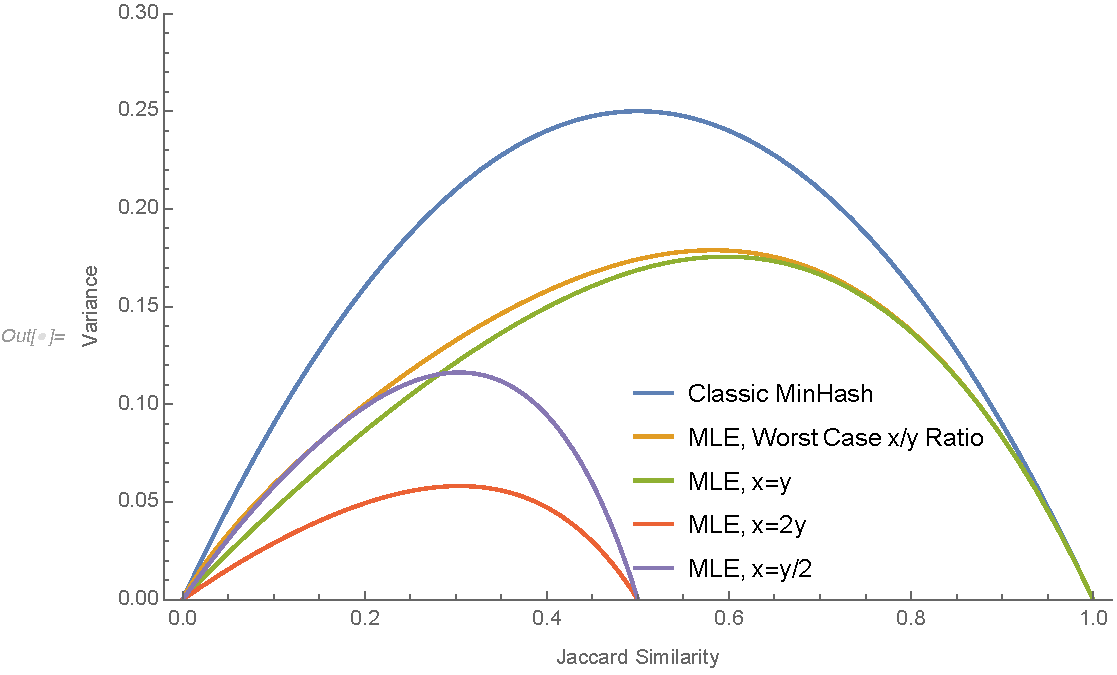
\includegraphics[trim=30 0 0 0,clip,width=\linewidth]{figures/mle_variance2}
\caption{Variance of Maximum Likelihood Estimator based on Fischer Information bound.
For $j$ close to 0 or 1 the worst case MLE bound is asymptotically equal to the Classical bound, whereas for $j\approx 0.21$ has only $\approx 62\%$ of the variance.}
\label{fig:mle_variance}
\end{figure}

The bound is a little complicated by the fact that it includes the sizes of the sets $n_x$ and $n_y$.
We note that the bound is convex in the ratio $n_y/n_x$, giving lower variances than \cref{eq:minvar} for $n_x<\!<n_y$ or $n_x >\!> n_y$.
\Cref{fig:mle_variance} shows \cref{eq:mle_var} when the ratio is taken to be \emph{worst possible}, as well as when it is taken to be 1
In the symmetric case $n_x=n_y$ the asymptotic variance reduces to
\[
   \frac{j(1-j)}{K}\frac{(1+j)^3}{2(1+3j)}.
\]
%for large $x$ and $y$.
For $n_x/n_y\neq1$ the Jaccard similarity is bounded above by $\frac{\min\{n_x,n_y\}}{\max\{n_x,n_y\}}$, which allows the MLE to discard those higher values from consideration.
Another interesting point from \cref{eq:mle_var} is that the variance at $n_x=c n_y$ is exactly $1/c$ of the variance at $n_x=n_y/c$.
It makes sense that the variance is lower when $|X|$ is big compared to $|Y|$, since we are given $X$, but don't know $Y$.

TODO: Stuff about local/global risk.
We can also compute the global risk of the MLE estimator, which is $0.178847/K$, $28.5\%$ less than the Classical Estimator.

\begin{proof}[Proof of \cref{prop:mle_var}]
   We first find the variance for the MLE estimator for $v$ and then show how to re-parametrize it to use the Jaccard similarity.

   Using Stirling's approximation $ \log n! = n\log n - n + O(\log n)$,
   we rewrite the log-likelihood \cref{eq:log-likelihood} as
   \begin{align}
      \ell(r;v) &=
      (x-k-[m\in x]+1)H(\tfrac{v-[m\in x]}{x-k-[m\in x]+1})
               - (x+1) H(\tfrac{v}{x+1})
              \\&+(u-m-[m\not\in x]-x+k+1) H(\tfrac{y-v-[m\not\in x]}{u-m-[m\not\in x]-x+k+1})
              \\& -(u-x+1) H(\tfrac{y-v}{u-x+1})
   + O(\log u),
   % TODO: We should probably also have error terms for n_y-v, n_x-v and so on.
   \end{align}
   where $H(p)=p \log \frac{1}{p} + (1-p)\log \frac{1}{1-p}$ is entropy function.

   Standard results~\cite{panchenko2016lec3} on Maximum Likelihood estimators say that
   the variance converges to $1/I(v)$ where
   \[
      I(v) = E\left[-\frac{d^2}{dv^2}\ell(m;v)\right]
   \]
   is known as the Fischer information.
   \footnote{This is actually a bit more tricky than it seems, since
      the standard proof of this fact~\cite{panchenko2016lec3} uses that the expectation is taken over the same probability space as $\ell$ is defined.
      However one can check that the key step in which that is used is to show
      $E[f''/f] = \int (f''(x)/f(x))f(x)dx = \int f''(dx) = (\int f(x)dx)'' = 0$, where $f=\exp(\ell)$ is the probability distribution.
      Since $E_h[f''/f] = E_h[E_{h_{|\overline X}}f''/f] = E_h[0]= 0$
      we can run the entire proof using $E_h$ rather than $E_{h_{|\overline X}}$ and get the same result.
      Thus it suffices to thus focus on bounding $E_h[-\frac{d^2}{dv^2}\ell(m;v)].
   % Something, something sigma algerba.
      % Basically I'm arguing that we can run the whole proof of MLE asymptotics and consider very expectatation as over $E_h$ rather than $E_{h_{|X}}$
   }

   % Strictly speaking the Fischer information is only defined when the log-likelihood is differentiable in the parameter $j$, which is not the case here, since we know $\frac{j}{1+j}(x+y)$ is an integer.

   %Since Stirling's approximation also applies to derivatives (simply exchanging the sum and the derivative operator)
   We can now evaluate the first two derivatives:
   {
      \thinmuskip=0mu
   \begin{align}
      % Single diff
      \frac{d}{dv}\ell(m;v)&=
   \log\left(\frac{(1-\frac1{y-v+1})^{[m\not\in x]}(1-\frac{k}{x-v+1})}{(1-\frac 1{v+1})^{[m\in x]}(1-\frac{m-k}{u-x-y+v+1})}\right) + O(1/u)
      \label{eq:deriv1}
      \\
      % Double diff
      \frac{d^2}{dv^2}\ell(m;v)&=
       [m\not\in x](\tfrac1{y-v+1}-\tfrac1{y-v})
      + (\tfrac1{x-v+1}-\tfrac1{x-v-k+1})
                               \\&
                               +[m\in x](\tfrac1{v+1}-\tfrac1{v})
      + (\tfrac1{u-x-y+v+1}-\tfrac1{u-x-y+v-m+k+1}) \\&+ O(1/u^2)
      \label{eq:deriv2}
      .
   \end{align}
   }

   There is something about the notation here.
   With $r\in x$ I mean thee probability that the smallest hash of $Y$ is in $X$.
   We now have three terms to bound:
   $E[r \in x]$, $\tfrac1{x-v-k+1}$ and $\tfrac1{u-x-y+v-m+k+1}$.
   The first is easy, since $m$ is a 

   Combining all the terms and assuming $x,y,u\to\infty$ we get
   \[
   I(v)
   = \frac{1}{y(x-v)} + \frac1{v(y-v)} + o(1/\min\{x,y\}).
   \]


   We can now use the reparemetrization formula for Fischer Information to compute
   \[
      I(j) = I(v)/j'(v)^2
   \]
   where $j(v) = v/(x-y+v)$.
   By the previously stated facts on Maximum Likelihood estimators, this proves the proposition.
\end{proof}


Relaxing this knowledge should only decrease the Fischer information (thus increase the variance) since we are throwing away somewhat useful information.

For twice differentiable $\ell(m;v)$,
the Fischer information is defined as
\[
   I(v) = -E[\frac{d^2}{dv^2}\ell(m;v)].
\]



%If $|x|=|y|=n$ that the variance $1/I(v)$ is maximized at $(\sqrt{2}-1)n$ with value $(\sqrt2-1)^2n^2$.
%That's cool.
%In general wee can get bounds like
%\[
   %V(X) \in [1-2\sqrt{2}/3, 1/16]\frac{m(4 xy-m^2)}{x},
%\]
%where $m=\min\{x,y\}$,
%or (the incomparible) $V(X) \le (\sqrt{2}-1)^2x^{1/2}y^{3/2}$.
%It is natural that we have some assymetry between $x$ and $y$, since that's the whole point of this paper.


Note that the variance of estimators usually depend on the answer.
This is known as Local Risk.
If we bound the variance by the worst possible parameter, in this case $j=1/2$ we get that the global risk of $1/(4K)$.

\subsection{Minner Estimator}

The starting point of this derivation is \cref{eq:deriv1},
to which we apply the approximation $\log(1-\eps) \approx -\eps$,
to get the equation
\[
   \frac{d}{dv}\ell(m;v) \approx
   -\frac{[m\not\in x]}{y-v} 
   -\frac{k}{x-v} 
   +\frac{[m\in x]}{v} 
   +\frac{m-k}{y-x-y+v} 
   = 0.
\]
When observing multiple $m_i's$, let $a=\sum_i [m\not\in x]$ and $b=\sum_i [m\in x]$.
Similarly let $k=\sum_i k_i$ and $m=\sum_i m_i$.
Then we want to solve
\[
   -\frac{a}{y-v} 
   -\frac{k}{x-v} 
   +\frac{b}{v} 
   +\frac{m-k}{y-x-y+v} 
   = 0.
\]
This can be rewritten as a degree three polynomial and solved by standard methods.
However, we would like a simpler estimator still.

In general we assume $u$ is very large, so we'll approximate $\frac{m-k}{u-x-y+v}\approx 0$.
If we further approximate $\frac{a}{y-v}\approx 0$ we get the simple solution $v=\frac{bx}{b+k}$.
This corresponds to the case where $v$ is small compared to $y$.
Alternatively, if we approximate $\frac{k}{x-v}\approx 0$, we get $v=\frac{b y}{a+b}$.
This corresponds to the case where $v$ is small compared to $x$.
From this intuition we propose the following estimator:
\begin{definition}[Minner Estimator]
\[
   T(m) = \min\left\{\frac{bx}{b+k}, \frac{b y}{a+b}\right\}.
   \label{eq:minner}
\]
\end{definition}
The resulting value is clearly always in the acceptable range $[0,\min\{x,y\}]$.

For Jaccard we do $j = v/(|X| + y - v)$

%Another thing: There may still be some cases where there is no solution within the acceptable range.
%I should probably do something about that?

We can improve upon the resulting estimate by Newton's method.
This is a common idea in MLE design. % TODO: Cite somebody?

TODO: I used to have some computations on this estimator as well...
Something like
\[
   E[\frac{bx}{b+k}] = \frac{v}{y} E[\frac{x}{1+k}]
\]
and so on.

\section{Old}


We start from the lower bound side by considering the Cramer Rao bound with $k=1$.
We define a random variable $Z$ to $\inf$ if $m\not\in x$ and $
= \sum_{z\in x\setminus y} [h(z) \le h(m)]$ otherwise.

Note that we can change the distribution of $h$ to be anything monotone without changing the probabilities.
We'll now assume it has exponential distribution.
%(Also note that that $\log 1/h(z)$ has exponential distribution.)
let $h^* = h(m)$, then $h^* = \min_{z\in y}h(z) \sim \text{Exp}(y)$ by stability of minimums.
We define $p=\Pr[h(z)\le h^*] = 1-\exp(-h^*)$.
Conditioning on $h^*$ we see that $Z$ has binomial distribution $B(n,p)$ where $n=|x\setminus y|$.

Back to the lower bound, 
Cramer Rao asks us to define
\[
   I(j) = E_{z,p}\left[\left(\frac{d\ell(z,p;\; j)}{d\ell}\right)^2\right]
\]
where (for $z\not=\inf$)
\begin{align}
   \exp(\ell(z;j))
   &=\Pr[Z=z]
 \\&= \Pr[m\in x]E_{h^*}[\binom{n}{z}p^z(1-p)^{n-z}]
 \\&= \tfrac{v}{y}E_{h^*}[\binom{n}{z} (1-e^{-h^*})^z e^{-h^*(n-z)}]
 \\&= \frac{v}{n+y}\binom{n}{z}\bigg/\binom{n+y-1}{z}
\end{align}
Approximating
\[
   \binom{n}{z}p^z(1-p)^{n-z} \sim \exp(-n D(z/n, p))
\]


Let's assume all the hash values on $x$ are fixed in advance.
Now we pick the values for $y\setminus x$.
We set $m=\argmin_{y_i\in y} h(y_i)$.
We are interested in the probability that $m\in x$ and $m=m^*$ for some element $m^*\in x\cap y$.
We define $h^*=h(m^*)$.

Let $Z$ be the minimum hash value in $y\setminus x$. Then it has distribution $\text{Exp}(|y|-v)$.
We are going to have $m=m^*$ exactly when $Z$ is larger than $h^*$.
(Such that no other value ``wins'' in $y$)
We also need $m$ to be the smallest in $x\cap y$, but that is implied by $m\in x$, since the hash values in $x$ are fixed.
Now $\Pr[Z \ge h^*] = \exp(h^*(|y|-v))$
so the total probability is $\frac{v}{y}\exp(-h^*(|y|-v))$.
This suggest the MLE of $v=-1/h^*$.
That can't be..

Maybe that whole combination argument is wrong.
Surely once we have $\Pr[Z\ge h^*]$ we already have $m\in x$, so we don't actually have that factor $v/y$...

What if I also use information when $m\not\in x$?
I can still compute the hash value of $m$ and compare it to my own hash values...
If $m\not\in x$ we have $Z < h^*$, where again $h^*$ is the smallest hash value in $x\cap y$.
This happens with probability $1-\exp(-h^*(|y|-v))$ which is most likely at $v=0$.
So this suggests a ``bang bang'' estimator, simply dependent on whether $m\in x$.
This is however still different from the normal minhash estimator, which also asks for the value to be smallest in $x$.

